% probsim.tex — companion paper for the probsim C99 library.
%
% Build with `make docs` (latexmk -pdf -bibtex).  Section numbers are load-
% bearing: the C sources cite them (e.g. src/dist.c refers to "paper §4.4"),
% and this paper cites the implementing file and function for everything it
% explains.  If you renumber sections, grep the sources for "paper" and fix
% the comments — README.md holds the master map.  The interactive web
% edition (docs/index.html) mirrors these sections too: keep its panel
% anchors in sync with the \webfig tags below, and re-copy the built PDF
% to docs/probsim.pdf after `make docs` (see README.md, "Web version").
\documentclass[11pt]{article}

\usepackage[a4paper,margin=2.6cm]{geometry}
\usepackage[T1]{fontenc}
\usepackage[utf8]{inputenc}
\usepackage{lmodern}
\usepackage{microtype}
\usepackage{amsmath,amssymb}
\usepackage{booktabs}
\usepackage{xcolor}
\usepackage{tikz}
\usetikzlibrary{arrows.meta,positioning,calc}
\usepackage{pgfplots}
\pgfplotsset{compat=1.18}
\usepackage[round]{natbib}

% ---- palette (validated for a white surface; see the repo's design notes) ----
\definecolor{sBlue}{HTML}{2A78D6}
\definecolor{sGreen}{HTML}{008300}
\definecolor{sMagenta}{HTML}{E87BA4}
\definecolor{sYellow}{HTML}{EDA100}
\definecolor{cRed}{HTML}{D03B3B}
\definecolor{inkP}{HTML}{0B0B0B}
\definecolor{inkS}{HTML}{52514E}
\definecolor{inkM}{HTML}{898781}
\definecolor{gridL}{HTML}{E1E0D9}
\definecolor{axisL}{HTML}{C3C2B7}

\usepackage[colorlinks=true,linkcolor=sBlue,citecolor=sGreen,urlcolor=sBlue]{hyperref}

\numberwithin{equation}{section}

% ---- shared figure styling: recessive axes, thin marks, direct labels ----
\pgfplotsset{
  psaxis/.style={
    width=10.6cm, height=5.6cm,
    axis lines=left,
    axis line style={axisL, semithick},
    every tick/.append style={axisL},
    ticklabel style={font=\scriptsize, color=inkM},
    xlabel style={font=\scriptsize\sffamily, color=inkS},
    ylabel style={font=\scriptsize\sffamily, color=inkS},
    ymajorgrids,
    grid style={gridL, very thin},
    every axis plot/.append style={line width=1.1pt},
    clip mode=individual,
  },
}
\tikzset{
  pslabel/.style={font=\scriptsize\sffamily, inner sep=1.5pt},
  dist/.style={rounded corners=2.5pt, font=\footnotesize\sffamily,
               text=white, inner sep=5pt, minimum height=6.5mm, draw=none},
  discretebox/.style={dist, fill=sGreen},
  contbox/.style={dist, fill=sBlue},
  rootbox/.style={dist, fill=sYellow, text=inkP},
  inferbox/.style={dist, fill=cRed},
  flow/.style={-{Stealth[length=2.4mm]}, semithick, color=inkM},
  flowlab/.style={font=\tiny\sffamily, color=inkS, fill=white,
                  inner sep=1.5pt, align=center},
}

% Inline pointer from a paper section to the code that implements it.
\newcommand{\srcref}[1]{%
  \par\smallskip\noindent{\small\sffamily\color{inkS}%
  $\hookrightarrow$ implemented in \texttt{#1}}\par\smallskip}

% The interactive web edition (docs/index.html), served via GitHub Pages
% from the sanya-shopper/distribs repository.
\newcommand{\siteurl}{https://sanya-shopper.github.io/distribs/}
% Tag for figure captions whose web counterpart is animated/interactive.
\newcommand{\webfig}[1]{{\small\sffamily\color{inkS}%
  [\href{\siteurl\##1}{interactive version on the web}]}}

\newcommand{\E}{\mathbb{E}}
\newcommand{\Var}{\operatorname{Var}}

\title{\textbf{Simulating the Classical Distributions}\\[2pt]
       \large A working tour from uniform bits to the $t$-test,\\
       with the \texttt{probsim} C99 library}
\author{The \texttt{probsim} project}
\date{July 2026}

\begin{document}
\maketitle

\begin{abstract}
\noindent
This paper accompanies \texttt{probsim}, a small C99 library that simulates
the twelve classical probability distributions and carries the results all
the way to working $t$-tests.  For each distribution we explain what it
models, where it earns its keep in statistical inference and applied
modeling, and how the library simulates it --- always with the simplest
algorithm that is still practical.  The distributions are presented as one
connected family (Figure~\ref{fig:family}): every sampler is built from
uniform bits, and the family funnels naturally into Student's $t$, whose
tail areas turn simulated or observed data into $p$-values.  Every section
names the source file and function that implements it, and the sources cite
these sections back, so paper and code can be read side by side.  This
paper also has \href{\siteurl}{an interactive web edition}
(\texttt{docs/index.html}, served via GitHub Pages) with every figure
animated --- each figure caption below links to its interactive
counterpart.
\end{abstract}

\section{Introduction}\label{sec:intro}

A probability distribution is a reusable answer to the question ``what does
this kind of randomness look like?''  A handful of them --- the
\emph{classical} distributions --- cover a remarkable share of practical
work: coin-like events, counts, waiting times, measurement noise, and the
sampling behaviour of statistics computed from data.  Learning them as
isolated formulas is hard; learning them as a \emph{family}, where each new
member is a short construction from ones you already know, is much easier.
That family view is exactly how the \texttt{probsim} library is written,
and Figure~\ref{fig:family} is its map.

\begin{figure}[htbp]
\centering
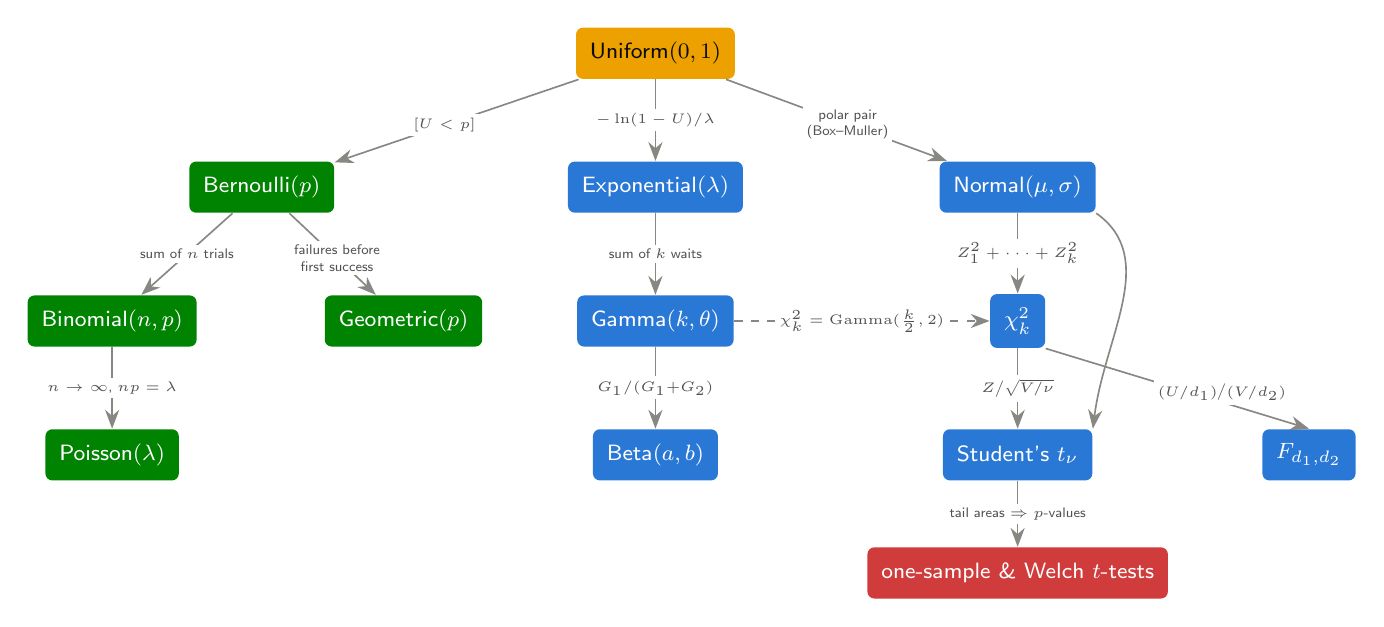
\begin{tikzpicture}[x=1cm, y=1cm]
  % root
  \node[rootbox] (unif) at (0.6,0) {Uniform$(0,1)$};
  % discrete branch (left)
  \node[discretebox] (bern) at (-4.4,-1.7) {Bernoulli$(p)$};
  \node[discretebox] (binom) at (-6.3,-3.4) {Binomial$(n,p)$};
  \node[discretebox] (geom) at (-2.6,-3.4) {Geometric$(p)$};
  \node[discretebox] (pois) at (-6.3,-5.1) {Poisson$(\lambda)$};
  % continuous branch (right)
  \node[contbox] (expo) at (0.6,-1.7) {Exponential$(\lambda)$};
  \node[contbox] (norm) at (5.2,-1.7) {Normal$(\mu,\sigma)$};
  \node[contbox] (gam) at (0.6,-3.4) {Gamma$(k,\theta)$};
  \node[contbox] (chi) at (5.2,-3.4) {$\chi^2_k$};
  \node[contbox] (beta) at (0.6,-5.1) {Beta$(a,b)$};
  \node[contbox] (stut) at (5.2,-5.1) {Student's $t_\nu$};
  \node[contbox] (fdist) at (8.9,-5.1) {$F_{d_1,d_2}$};
  % inference sink
  \node[inferbox] (ttest) at (5.2,-6.6) {one-sample \& Welch $t$-tests};
  % edges
  \draw[flow] (unif) -- (bern)
    node[flowlab, pos=0.55] {$[U<p]$};
  \draw[flow] (bern) -- (binom)
    node[flowlab, pos=0.5] {sum of $n$ trials};
  \draw[flow] (bern) -- (geom)
    node[flowlab, pos=0.55] {failures before\\first success};
  \draw[flow] (binom) -- (pois)
    node[flowlab, pos=0.5] {$n\to\infty$, $np=\lambda$};
  \draw[flow] (unif) -- (expo)
    node[flowlab, pos=0.5] {$-\ln(1-U)/\lambda$};
  \draw[flow] (unif) -- (norm)
    node[flowlab, pos=0.55] {polar pair\\(Box--Muller)};
  \draw[flow] (expo) -- (gam)
    node[flowlab, pos=0.5] {sum of $k$ waits};
  \draw[flow] (norm) -- (chi)
    node[flowlab, pos=0.5] {$Z_1^2+\cdots+Z_k^2$};
  \draw[flow, dashed] (gam) -- (chi)
    node[flowlab, pos=0.5] {$\chi^2_k=\mathrm{Gamma}(\tfrac{k}{2},2)$};
  \draw[flow] (gam) -- (beta)
    node[flowlab, pos=0.5] {$G_1/(G_1{+}G_2)$};
  \draw[flow] (norm.south east) .. controls (7.0,-2.6) and (6.3,-3.6) ..
    (stut.north east);
  \draw[flow] (chi) -- (stut)
    node[flowlab, pos=0.5] {$Z\big/\sqrt{V/\nu}$};
  \draw[flow] (chi.south east) -- (fdist.north)
    node[flowlab, pos=0.55, xshift=4mm] {$(U/d_1)\big/(V/d_2)$};
  \draw[flow] (stut) -- (ttest)
    node[flowlab, pos=0.5] {tail areas $\Rightarrow$ $p$-values};
\end{tikzpicture}
\caption{The classical family as \texttt{probsim} builds it.  Everything
starts from uniform bits (\S\ref{sec:rng}); \textcolor{sGreen}{discrete}
distributions grow along the left (\S\ref{sec:discrete}),
\textcolor{sBlue}{continuous} ones along the right (\S\ref{sec:continuous}),
and the family funnels into the \textcolor{cRed}{$t$-tests} of
\S\ref{sec:inference}.  Each arrow is literally a line or two of C in
\texttt{src/dist.c}.\ \webfig{family}}
\label{fig:family}
\end{figure}

\paragraph{How to read this with the code.}
The library is four small C files behind one header,
\texttt{include/probsim.h}.  Section \S\ref{sec:rng} covers
\texttt{src/rng.c}; \S\ref{sec:discrete} and \S\ref{sec:continuous} cover
\texttt{src/dist.c}; \S\ref{sec:inference} covers \texttt{src/special.c}
and \texttt{src/stats.c}; \S\ref{sec:driver} walks through the driver
\texttt{app/simulate.c} and the test suite \texttt{tests/test\_probsim.c}.
Each subsection below ends with a pointer to its implementation, and the
source comments point back here.  Throughout, the guiding rule is the one
this library was written under: \emph{prefer the simplest algorithm that is
easy to understand and still practical to use}.  Where a cleverer method is
the industry standard --- the ziggurat for normals, say
\citep{marsaglia2000ziggurat} --- we cite it, explain the trade-off, and
keep the simple one.

\section{Where the randomness comes from}\label{sec:rng}

Computers are deterministic, so ``random'' numbers are produced by a
\emph{pseudo-random number generator} (PRNG): a small state machine whose
output sequence is indistinguishable, for statistical purposes, from true
randomness.  \texttt{probsim} uses \textbf{xoshiro256++}
\citep{blackman2021xoshiro}: 256 bits of state, a period of $2^{256}-1$,
excellent results on the standard test batteries, and a step function of
about ten lines --- comfortably inside our simplicity rule.  Reasonable
alternatives with the same spirit include PCG \citep{oneill2014pcg}; the
deeper theory of testing generators is in \citet[ch.~3]{knuth1997}.  None
of these are cryptographic generators, and \texttt{probsim} should never be
used where an adversary matters.

Two practical details deserve attention because they bite working
statisticians.  First, \emph{seeding}: naive seeds like $1, 2, 3$ are
nearly identical bit patterns, and a weak seeding routine would start the
streams in correlated states.  The library therefore runs every seed
through the splitmix64 mixer, as the xoshiro authors recommend.  Second,
\emph{explicit state}: every sampler takes a \texttt{ps\_rng~*} argument
and there is no hidden global, so a simulation is reproducible from a
single recorded seed and independent streams are just independent structs
--- which is what makes the test suite of \S\ref{sec:driver} deterministic.

\subsection{Uniform is enough}\label{sec:uniform-enough}

The raw generator emits 64-bit integers; dividing the top 53 bits by
$2^{53}$ gives a double $U$ uniform on $[0,1)$ at full mantissa precision.
Everything else in this paper is manufactured from such $U$'s.  The
master tool is \emph{inverse-transform sampling}: if $F$ is a CDF and
$U\sim\mathrm{Uniform}(0,1)$, then $X=F^{-1}(U)$ has CDF exactly $F$,
because $\Pr[X\le x]=\Pr[U\le F(x)]=F(x)$.  Figure~\ref{fig:inverse} shows
the idea; the exponential sampler of \S\ref{sec:exponential} is its
purest one-line application.  When $F^{-1}$ is awkward, two other levers
--- \emph{transformation} (build the variable from simpler ones) and
\emph{rejection} (propose, then accept with the right probability) ---
take over; both appear in \S\ref{sec:continuous}.  The encyclopedia of
all three techniques is \citet{devroye1986}.

\begin{figure}[htbp]
\centering
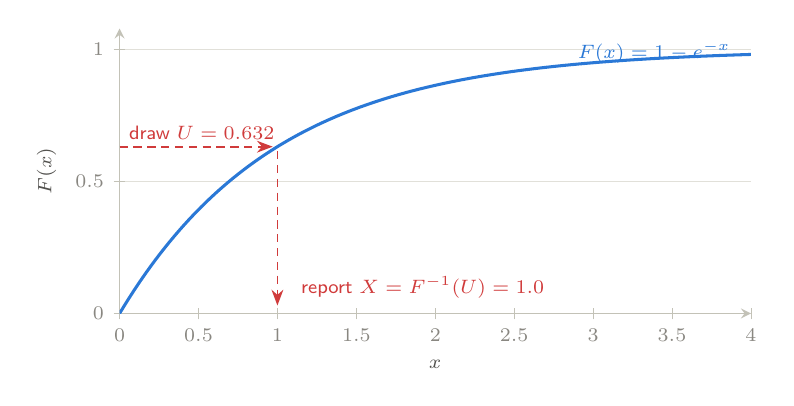
\begin{tikzpicture}
\begin{axis}[psaxis, width=9.6cm, height=5.2cm,
    xmin=0, xmax=4, ymin=0, ymax=1.08,
    xlabel={$x$}, ylabel={$F(x)$},
    domain=0:4, samples=140]
  \addplot[sBlue] {1-exp(-x)};
  \node[pslabel, color=sBlue, anchor=south east] at (axis cs:3.9,0.93)
    {$F(x)=1-e^{-x}$};
  \draw[-{Stealth[length=2mm]}, cRed, semithick, densely dashed]
    (axis cs:0,0.632) -- (axis cs:0.97,0.632);
  \draw[-{Stealth[length=2mm]}, cRed, semithick, densely dashed]
    (axis cs:1.0,0.615) -- (axis cs:1.0,0.03);
  \node[pslabel, color=cRed, anchor=south west] at (axis cs:0.03,0.64)
    {draw $U=0.632$};
  \node[pslabel, color=cRed, anchor=west] at (axis cs:1.12,0.10)
    {report $X=F^{-1}(U)=1.0$};
\end{axis}
\end{tikzpicture}
\caption{Inverse-transform sampling: a uniform draw on the vertical axis is
pushed through $F^{-1}$ to land on the horizontal axis with density exactly
$F'$.  Regions where $F$ rises steeply receive more of the uniform mass ---
that is the whole trick.\ \webfig{uniform-bits}}
\label{fig:inverse}
\end{figure}

\srcref{src/rng.c: ps\_rng\_seed(), ps\_rng\_next(), ps\_runif()}

\section{The discrete family}\label{sec:discrete}

Discrete distributions describe counts.  The four classical ones form a
single story: a yes/no event (Bernoulli), how many yeses in $n$ tries
(binomial), how long until the first yes (geometric), and how many events
occur when opportunities are numerous but each is rare (Poisson).  The
driver \texttt{app/simulate.c} exercises each with the worked parameters
used below.

\subsection{Bernoulli}\label{sec:bernoulli}

The Bernoulli$(p)$ variable is a single yes/no experiment:
$\Pr[X{=}1]=p$, $\Pr[X{=}0]=1-p$, with $\E X = p$ and $\Var X = p(1-p)$.
It is the atom of applied statistics: a conversion in an A/B test, a
defective part, a patient responding to treatment, a loan defaulting.
Almost all of \emph{binary-outcome} inference --- estimating a proportion,
comparing two proportions, logistic regression --- is Bernoulli modeling.
Simulation is the definition itself: draw $U$ and report whether $U<p$.

\srcref{src/dist.c: ps\_bernoulli()}

\subsection{Binomial}\label{sec:binomial}

The Binomial$(n,p)$ variable counts successes in $n$ independent
Bernoulli$(p)$ trials:
\[
\Pr[X=k]=\binom{n}{k}p^k(1-p)^{\,n-k},\qquad
\E X = np,\quad \Var X = np(1-p).
\]
It models any fixed-quota count: heads in $n$ tosses, positive responses
among $n$ patients, defects in a batch of $n$ (the basis of industrial
\emph{acceptance sampling}), conversions among $n$ visitors.  In
inference it is the exact sampling distribution behind every test of a
proportion --- the sign test, the exact binomial test, and, through the
normal approximation, the familiar $z$-test for proportions.
\texttt{probsim} simulates it as what it is --- $n$ Bernoulli draws summed
--- an $O(n)$ loop that cannot be wrong by inspection; sub-linear samplers
exist \citep[ch.~X.4]{devroye1986} but buy speed with complexity we do not
need.  Figure~\ref{fig:pmfs} (left) shows the worked example
Binomial$(20, 0.25)$.

\srcref{src/dist.c: ps\_binomial(), ps\_binomial\_pmf()}

\subsection{Geometric}\label{sec:geometric}

The Geometric$(p)$ variable counts \emph{failures before the first
success} (support $0,1,2,\dots$, the convention of R's \texttt{rgeom}):
$\Pr[X=k]=p(1-p)^k$, $\E X=(1-p)/p$, $\Var X=(1-p)/p^2$.  It is the
discrete waiting time: retries before a packet gets through, cold calls
before a sale, coin flips before the first head.  Its \emph{memoryless}
property (past failures tell you nothing about the future) makes it the
discrete twin of the exponential --- and indeed the sampler exploits
exactly that: invert the geometric CDF with one uniform,
$X=\lfloor \ln(1-U)/\ln(1-p)\rfloor$, which is the exponential inversion
of \S\ref{sec:exponential} rounded down to a count.

\srcref{src/dist.c: ps\_geometric(), ps\_geometric\_pmf()}

\subsection{Poisson}\label{sec:poisson}

The Poisson$(\lambda)$ variable is the law of rare events: the limit of
Binomial$(n, \lambda/n)$ as $n\to\infty$,
\[
\Pr[X=k]=e^{-\lambda}\frac{\lambda^k}{k!},\qquad
\E X=\Var X=\lambda .
\]
It models counts per unit of exposure when events are individually
unlikely but opportunities are many: arrivals at a queue per minute,
radioactive decays per second, typos per page, insurance claims per
policy-year, sequencing reads per gene.  In inference it anchors count
regression (Poisson GLMs, with the $\E X=\Var X$ property serving as the
canonical check for \emph{overdispersion}) and classical goodness-of-fit
tests.  The library simulates it with Knuth's product-of-uniforms method
\citep[\S3.4.1]{knuth1997} --- count uniforms until their running product
drops below $e^{-\lambda}$ --- applied in chunks of rate at most 30 so the
product never underflows; the chunking is valid because Poisson rates add.
Figure~\ref{fig:pmfs} (right) shows Poisson$(4)$.

\begin{figure}[htbp]
\centering
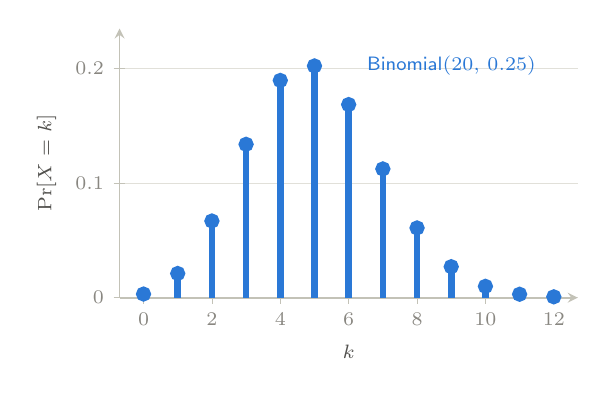
\begin{tikzpicture}
\begin{axis}[psaxis, width=7.4cm, height=5.0cm,
    xmin=-0.7, xmax=12.7, ymin=0, ymax=0.235,
    xlabel={$k$}, ylabel={$\Pr[X=k]$}]
  \addplot[ycomb, sBlue, line width=2.4pt, mark=*, mark size=1.5pt]
    coordinates {(0,0.003171) (1,0.021141) (2,0.066948) (3,0.133896)
      (4,0.189685) (5,0.202331) (6,0.168609) (7,0.112406) (8,0.060887)
      (9,0.027061) (10,0.009922) (11,0.003007) (12,0.000752)};
  \node[pslabel, color=sBlue, anchor=south west] at (axis cs:6.4,0.19)
    {Binomial$(20,\,0.25)$};
\end{axis}
\end{tikzpicture}\hfill
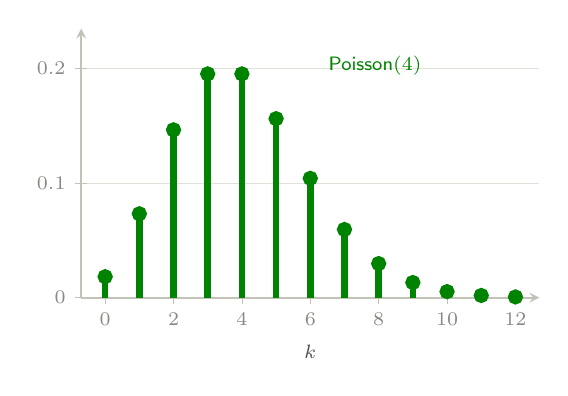
\begin{tikzpicture}
\begin{axis}[psaxis, width=7.4cm, height=5.0cm,
    xmin=-0.7, xmax=12.7, ymin=0, ymax=0.235,
    xlabel={$k$}, ylabel={}]
  \addplot[ycomb, sGreen, line width=2.4pt, mark=*, mark size=1.5pt]
    coordinates {(0,0.018316) (1,0.073263) (2,0.146525) (3,0.195367)
      (4,0.195367) (5,0.156293) (6,0.104196) (7,0.059540) (8,0.029770)
      (9,0.013231) (10,0.005292) (11,0.001925) (12,0.000642)};
  \node[pslabel, color=sGreen, anchor=south west] at (axis cs:6.4,0.19)
    {Poisson$(4)$};
\end{axis}
\end{tikzpicture}
\caption{The two classical count laws, at the driver's worked parameters.
Both have mean $\approx 4$--$5$, but the binomial is confined to
$\{0,\dots,20\}$ while the Poisson has an unbounded right tail --- the
visible signature of ``many opportunities, each rare''.\ \webfig{discrete}}
\label{fig:pmfs}
\end{figure}

\srcref{src/dist.c: ps\_poisson(), ps\_poisson\_pmf()}

\section{The continuous family}\label{sec:continuous}

Continuous distributions describe measurements.  We meet them in the order
the library constructs them (the right-hand side of
Figure~\ref{fig:family}), because each is a short recipe from the previous
ones.

\subsection{Uniform}\label{sec:uniform}

Uniform$(a,b)$ spreads its mass evenly: density $1/(b-a)$ on $[a,b)$, mean
$(a+b)/2$, variance $(b-a)^2/12$.  Beyond being the raw material of
\S\ref{sec:uniform-enough}, it is a model in its own right (rounding
error, phases, arrival offsets) and a cornerstone of inference through one
beautiful fact: \emph{under a true null hypothesis, a $p$-value is
Uniform$(0,1)$}.  That fact is testable --- the test suite verifies it
empirically in \S\ref{sec:tests} --- and it underlies $p$-value histograms,
false-discovery-rate methods, and simulation-based calibration.
Simulation is one affine map of $U$.

\srcref{src/dist.c: ps\_uniform()}

\subsection{Exponential}\label{sec:exponential}

The Exponential$(\lambda)$ variable (rate $\lambda$; density
$\lambda e^{-\lambda x}$, mean $1/\lambda$, variance $1/\lambda^2$) is the
continuous waiting time to the next event of a constant-rate process ---
the continuous twin of the geometric, and like it \emph{memoryless}: a
component that has survived $t$ hours is statistically as good as new.
That property makes it the baseline model of reliability engineering,
queueing theory (service and inter-arrival times), and survival analysis,
where its constant \emph{hazard rate} is the reference against which
ageing (or infant-mortality) effects are measured.  The sampler is the
one-liner promised in Figure~\ref{fig:inverse}:
$X=-\ln(1-U)/\lambda$.

\srcref{src/dist.c: ps\_exponential(), ps\_exponential\_cdf()}

\subsection{Normal}\label{sec:normal}

The Normal$(\mu,\sigma)$ density
$\frac{1}{\sigma\sqrt{2\pi}}e^{-(x-\mu)^2/2\sigma^2}$ is the center of
gravity of statistics, for one overwhelming reason: the \emph{central
limit theorem}.  Sums and averages of many small independent effects are
approximately normal almost regardless of the ingredients' own
distributions --- which is why measurement errors, biological traits, and
sample means all look Gaussian, and why the normal is the default model
for noise in regression and the reference distribution for estimators.
Essentially all of \S\ref{sec:inference} exists to make small-sample
corrections to normal-based reasoning.

$F^{-1}$ has no closed form, so inversion is unavailable; instead the
library uses the polar variant of the Box--Muller transform
\citep{boxmuller1958}, our one \emph{rejection} sampler
(Figure~\ref{fig:polar}): draw $(v_1,v_2)$ uniformly in the square
$[-1,1]^2$, accept when $s=v_1^2+v_2^2<1$ (probability $\pi/4\approx
79\%$), and return $v_1\sqrt{-2\ln s / s}$, which is exactly standard
normal.\footnote{The method actually yields \emph{two} independent
normals, $v_1\sqrt{-2\ln s/s}$ and $v_2\sqrt{-2\ln s/s}$;
\texttt{ps\_normal()} discards the second so the sampler carries no state
between calls.  Production libraries chasing speed instead use the
ziggurat method \citep{marsaglia2000ziggurat}, a heavily engineered
rejection scheme --- a good example of the complexity our simplicity rule
declines.}

\begin{figure}[htbp]
\centering
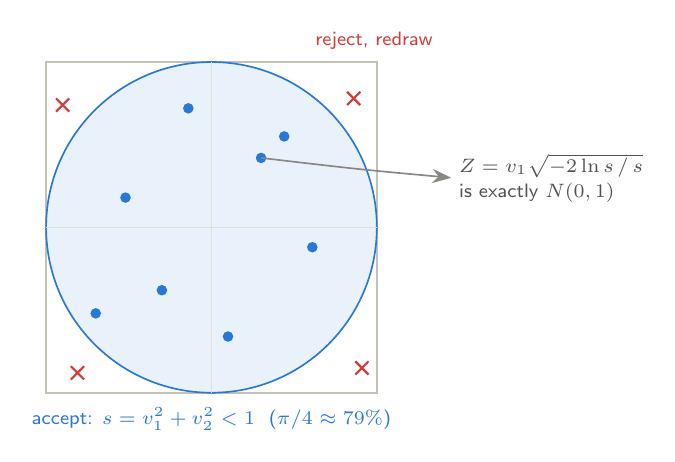
\begin{tikzpicture}[scale=2.1]
  \draw[axisL, semithick] (-1,-1) rectangle (1,1);
  \fill[sBlue, fill opacity=0.10] (0,0) circle (1);
  \draw[sBlue, semithick] (0,0) circle (1);
  \draw[gridL, very thin] (-1,0) -- (1,0);
  \draw[gridL, very thin] (0,-1) -- (0,1);
  % accepted points
  \foreach \x/\y in {0.30/0.42, -0.52/0.18, 0.10/-0.66, -0.30/-0.38,
                     0.61/-0.12, -0.14/0.72, 0.44/0.55, -0.70/-0.52}
    \fill[sBlue] (\x,\y) circle (0.032);
  % rejected points
  \foreach \x/\y in {0.86/0.78, -0.90/0.74, 0.91/-0.85, -0.81/-0.88}
    \draw[cRed, thick] (\x-0.04,\y-0.04) -- (\x+0.04,\y+0.04)
                       (\x-0.04,\y+0.04) -- (\x+0.04,\y-0.04);
  \node[pslabel, color=sBlue, anchor=north] at (0,-1.06)
    {accept: $s=v_1^2+v_2^2<1$ \ ($\pi/4\approx79\%$)};
  \node[pslabel, color=cRed, anchor=south west] at (0.6,1.05)
    {reject, redraw};
  \draw[flow] (0.30,0.42) .. controls (0.9,0.35) .. (1.45,0.30);
  \node[pslabel, color=inkS, anchor=west, align=left] at (1.47,0.30)
    {$Z = v_1\sqrt{-2\ln s\,/\,s}$\\[1pt] is exactly $N(0,1)$};
\end{tikzpicture}
\caption{The polar Box--Muller sampler: uniform points in the square are
kept only if they land in the disc; the kept point's radius and direction
are then reshaped into a standard normal.  Rejection turns an easy
distribution (uniform on a square) into a hard one (uniform on a disc)
at a known, modest cost.\ \webfig{normal}}
\label{fig:polar}
\end{figure}

\srcref{src/dist.c: ps\_normal(), ps\_normal\_pdf(), ps\_normal\_cdf()}

\subsection{Gamma}\label{sec:gamma}

The Gamma$(k,\theta)$ family (shape $k$, scale $\theta$; density
$\propto x^{k-1}e^{-x/\theta}$, mean $k\theta$, variance $k\theta^2$) is
the flexible law of \emph{accumulated} waiting: for integer $k$ it is
exactly the time until the $k$-th event of a Poisson process --- a sum of
$k$ exponentials --- and general $k$ interpolates smoothly
(Figure~\ref{fig:gamma}).  It models rainfall totals, insurance losses,
service times, and neuronal inter-spike intervals; in Bayesian inference
it is the conjugate prior for Poisson and exponential rates, so posterior
simulation of rate parameters is gamma sampling.  It also generates the
next two distributions outright.

Summing exponentials only works for integer $k$, so the library uses the
one algorithm where we accept a little cleverness for a lot of practical
value: the \citet{marsaglia2000gamma} method, the standard choice of
modern statistical software, and still only a dozen lines.  Its idea is a
polished version of Figure~\ref{fig:polar}'s: push a normal draw $Z$
through the smooth cube $X=d(1+Z/\sqrt{9d})^3$ with $d=k-\tfrac13$, which
lands \emph{almost} exactly on the gamma density, then repair the small
discrepancy with a rejection step that accepts well over 95\% of
proposals.  Shapes $k<1$ (where the density blows up at zero) are handled
by a classical boost: draw at shape $k+1$ and multiply by $U^{1/k}$.

\begin{figure}[htbp]
\centering
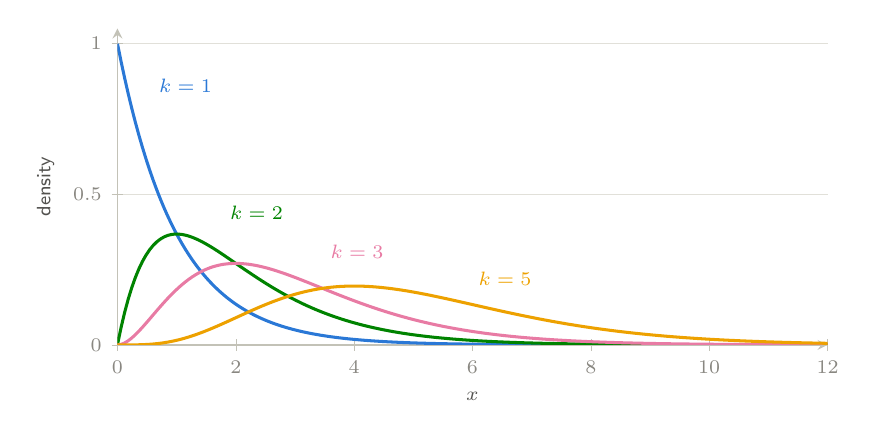
\begin{tikzpicture}
\begin{axis}[psaxis, xmin=0, xmax=12, ymin=0, ymax=1.05,
    xlabel={$x$}, ylabel={density}, domain=0.001:12, samples=200]
  \addplot[sBlue]    {exp(-x)};
  \addplot[sGreen]   {x*exp(-x)};
  \addplot[sMagenta] {0.5*x^2*exp(-x)};
  \addplot[sYellow]  {x^4*exp(-x)/24};
  \node[pslabel, color=sBlue]    at (axis cs:1.15,0.86) {$k=1$};
  \node[pslabel, color=sGreen]   at (axis cs:2.35,0.44) {$k=2$};
  \node[pslabel, color=sMagenta] at (axis cs:4.05,0.31) {$k=3$};
  \node[pslabel, color=sYellow]  at (axis cs:6.55,0.22) {$k=5$};
\end{axis}
\end{tikzpicture}
\caption{Gamma densities with scale $\theta=1$.  Shape $k=1$ is the
exponential; as $k$ grows the density moves right, symmetrizes, and (by
the CLT, since it is a sum of $k$ waits) approaches a normal --- the
family tree of Figure~\ref{fig:family} in a single picture.\
\webfig{gamma}}
\label{fig:gamma}
\end{figure}

\srcref{src/dist.c: ps\_gamma(), ps\_gamma\_cdf()}

\subsection{Beta}\label{sec:beta}

The Beta$(a,b)$ family lives on $(0,1)$ with density
$\propto x^{a-1}(1-x)^{b-1}$, mean $a/(a{+}b)$, and variance
$ab/\!\left((a{+}b)^2(a{+}b{+}1)\right)$; its shapes
(Figure~\ref{fig:beta}) run from uniform through unimodal humps to
J- and U-curves.  It is \emph{the} distribution for unknown proportions:
in Bayesian inference it is the conjugate prior for the Bernoulli/binomial
$p$ --- start from Beta$(a,b)$, observe $s$ successes and $f$ failures,
and the posterior is Beta$(a{+}s,\,b{+}f)$, which is why Thompson-sampling
bandits and Bayesian A/B testing are, computationally, beta simulation.
It also models proportions directly (beta regression) and is the order-%
statistics law: the $k$-th smallest of $n$ uniforms is
Beta$(k,\,n{-}k{+}1)$.  The sampler uses the classical gamma
representation: $X=G_1/(G_1+G_2)$ with independent
$G_1\sim\mathrm{Gamma}(a,1)$, $G_2\sim\mathrm{Gamma}(b,1)$.

\begin{figure}[htbp]
\centering
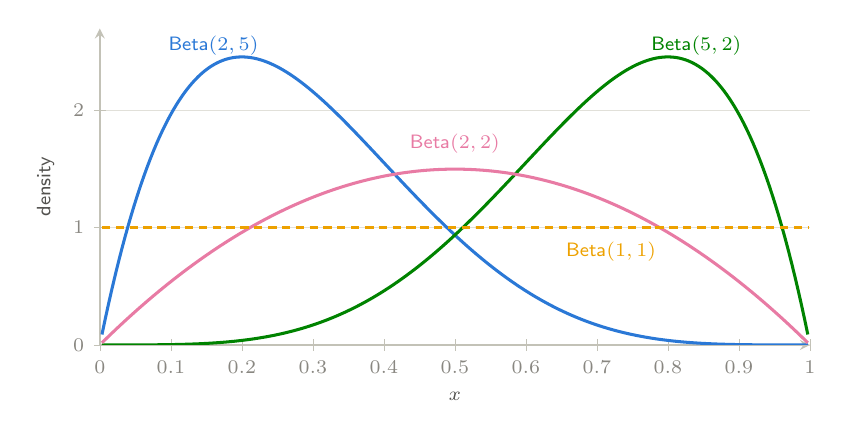
\begin{tikzpicture}
\begin{axis}[psaxis, xmin=0, xmax=1, ymin=0, ymax=2.7,
    xlabel={$x$}, ylabel={density}, domain=0.003:0.997, samples=220]
  \addplot[sBlue]    {30*x*(1-x)^4};
  \addplot[sGreen]   {30*x^4*(1-x)};
  \addplot[sMagenta] {6*x*(1-x)};
  \addplot[sYellow, densely dashed]  {1};
  \node[pslabel, color=sBlue]    at (axis cs:0.16,2.55) {Beta$(2,5)$};
  \node[pslabel, color=sGreen]   at (axis cs:0.84,2.55) {Beta$(5,2)$};
  \node[pslabel, color=sMagenta] at (axis cs:0.5,1.72)  {Beta$(2,2)$};
  \node[pslabel, color=sYellow]  at (axis cs:0.72,0.80) {Beta$(1,1)$};
\end{axis}
\end{tikzpicture}
\caption{Beta densities: the driver's worked example Beta$(2,5)$ leans
toward small proportions, its mirror Beta$(5,2)$ toward large ones,
Beta$(2,2)$ is a symmetric hump, and Beta$(1,1)$ is the uniform ---
the natural ``know nothing'' prior for a probability.\ \webfig{beta}}
\label{fig:beta}
\end{figure}

\srcref{src/dist.c: ps\_beta(), ps\_beta\_cdf()}

\subsection{Chi-squared}\label{sec:chisq}

The $\chi^2_k$ variable is a sum of $k$ squared standard normals; it is
also exactly Gamma$(k/2,\,2)$, which is how the library both simulates it
(one call to \texttt{ps\_gamma}) and evaluates its CDF.  Mean $k$,
variance $2k$.  Its starring role is as the \emph{distribution of
accumulated squared noise}: in a normal sample of size $n$, the rescaled
sample variance $(n-1)S^2/\sigma^2$ is $\chi^2_{n-1}$ --- the fact that
makes confidence intervals for variances possible and, in the next
section, gives the $t$ statistic its denominator.  It reappears wherever
squared deviations are summed: Pearson's goodness-of-fit and
independence tests, and the asymptotic null distribution of
likelihood-ratio statistics (Wilks' theorem) --- which makes $\chi^2$
tail areas the common currency of model comparison.

\srcref{src/dist.c: ps\_chi\_squared(), ps\_chi\_squared\_cdf()}

\subsection{Student's t}\label{sec:studentt}

Student's $t_\nu$ is defined by the construction at the heart of this
library:
\[
T=\frac{Z}{\sqrt{V/\nu}},\qquad Z\sim N(0,1),\quad V\sim\chi^2_\nu
\text{ independent},
\]
and the sampler is that definition verbatim.  It looks like a normal but
with \emph{heavier tails} (Figure~\ref{fig:tvsn}): dividing by an
estimated, rather than known, scale injects extra uncertainty, and the
smaller $\nu$ is, the fatter the tails.  As $\nu\to\infty$ it converges to
the normal; at $\nu=1$ it is the wild Cauchy with no mean at all.
Historically it was discovered by \citet{student1908} --- W.~S.~Gosset,
publishing pseudonymously from the Guinness brewery --- precisely because
brewery samples were too small for large-sample normal theory.  Beyond
the $t$-tests of \S\ref{sec:inference} (and the confidence intervals
$\bar x \pm t_{\nu}^{*}\,s/\sqrt n$ dual to them), its heavy tails make
it a workhorse \emph{model} in its own right: robust regression replaces
normal errors with $t$ errors so outliers stop dragging the fit, and
finance uses $t$ innovations because asset returns produce extreme moves
far more often than a Gaussian allows.

\begin{figure}[htbp]
\centering
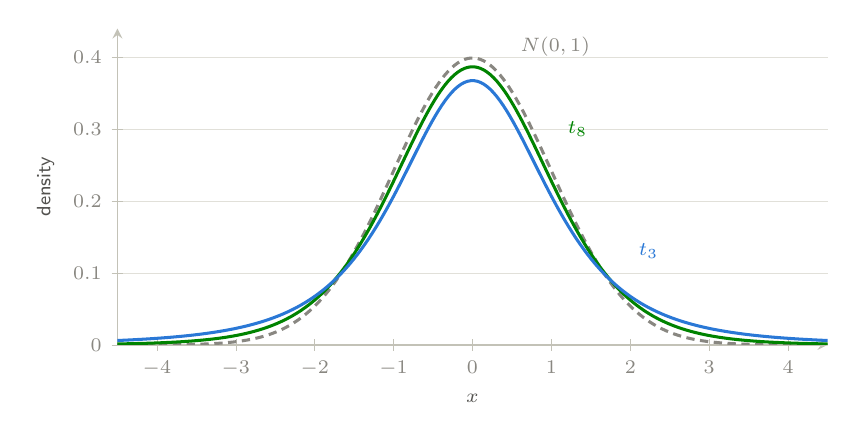
\begin{tikzpicture}
\begin{axis}[psaxis, xmin=-4.5, xmax=4.5, ymin=0, ymax=0.44,
    xlabel={$x$}, ylabel={density}, domain=-4.5:4.5, samples=220]
  \addplot[inkM, densely dashed] {0.3989423*exp(-x^2/2)};
  \addplot[sGreen] {0.3866990*(1+x^2/8)^(-4.5)};
  \addplot[sBlue]  {0.3675526*(1+x^2/3)^(-2)};
  \node[pslabel, color=inkM,   anchor=west] at (axis cs:0.55,0.415)
    {$N(0,1)$};
  \node[pslabel, color=sGreen, anchor=west] at (axis cs:1.15,0.30)
    {$t_8$};
  \node[pslabel, color=sBlue,  anchor=west] at (axis cs:2.05,0.13)
    {$t_3$};
\end{axis}
\end{tikzpicture}
\caption{Student's $t$ against the standard normal.  The lower the degrees
of freedom, the more probability escapes into the tails --- so small
samples need larger observed effects before a result counts as
surprising.  This gap between $t_\nu$ and $N(0,1)$ \emph{is} the
small-sample correction of \S\ref{sec:inference}.\ \webfig{studentt}}
\label{fig:tvsn}
\end{figure}

\srcref{src/dist.c: ps\_student\_t(), ps\_student\_t\_pdf(),
        ps\_student\_t\_cdf()}

\subsection{Fisher's F}\label{sec:f}

The $F_{d_1,d_2}$ variable is a ratio of independent normalized
chi-squareds, $F=(U/d_1)/(V/d_2)$ --- the sampler, once again, is the
definition.  Since sample variances are scaled chi-squareds
(\S\ref{sec:chisq}), $F$ is the natural null distribution for
\emph{comparing variances}: its tail areas power the classical ANOVA
$F$-test (is the variance \emph{between} group means larger than the
variance \emph{within} groups?), the overall significance test of a
regression, and nested-model comparisons.  Two connections knit the
family shut: $t_\nu^2 = F_{1,\nu}$ (squaring a $t$-test gives an
$F$-test), and ANOVA with two groups is exactly the pooled $t$-test.

\srcref{src/dist.c: ps\_f(), ps\_f\_cdf()}

\section{From distributions to inference: the t-test}\label{sec:inference}

Everything so far generated data; this section reasons \emph{backwards}
from data.  The $t$-test is the classical family's flagship application,
and its logic recurs across all of statistics: reduce the data to a
statistic whose distribution under a null hypothesis is known exactly
(here, thanks to \S\ref{sec:normal}--\S\ref{sec:studentt}), then ask how
extreme the observed value is under that distribution.

\subsection{Two special functions carry all the tables}
\label{sec:special}

Before software, the answer to ``how extreme?'' lived in printed tables at
the back of textbooks.  All of those tables compress into two special
functions.  The \emph{regularized incomplete beta function}
\begin{equation}\label{eq:incbeta}
I_x(a,b)=\frac{1}{B(a,b)}\int_0^x u^{a-1}(1-u)^{b-1}\,du ,
\end{equation}
is the beta CDF, and the $t$ and $F$ CDFs reduce to it algebraically; for
the $t$,
\begin{equation}\label{eq:tcdf}
\Pr[T_\nu\le t] \;=\; 1-\tfrac12\,
I_{\frac{\nu}{\nu+t^2}}\!\Bigl(\tfrac{\nu}{2},\tfrac12\Bigr)
\qquad (t\ge 0),
\end{equation}
with the $t<0$ case supplied by symmetry, and
$\Pr[F_{d_1,d_2}\le x] = I_{d_1x/(d_1x+d_2)}(d_1/2,\,d_2/2)$.  Its
sibling, the \emph{regularized lower incomplete gamma function}
$P(a,x)=\frac{1}{\Gamma(a)}\int_0^x u^{a-1}e^{-u}\,du$, is the gamma CDF
and hence the chi-squared and Poisson tail machinery.  \texttt{probsim}
evaluates both with the classical series/continued-fraction pairs
\citep[\S6.2, \S6.4]{press1992}, accurate to about $10^{-14}$ ---
each roughly forty lines of C that replace every table in the book.

\srcref{src/special.c: ps\_incbeta(), ps\_incgamma\_lower()}

\subsection{The one-sample t-test}\label{sec:onesample}

Model $n$ observations as $X_i \sim N(\mu,\sigma^2)$ with both parameters
unknown, and test $H_0\colon \mu=\mu_0$.  Three facts from
\S\ref{sec:continuous} assemble the test.  Under $H_0$: (i)
$\bar X \sim N(\mu_0, \sigma^2/n)$; (ii)
$(n-1)S^2/\sigma^2 \sim \chi^2_{n-1}$, where $S^2$ is the sample variance
with the $n-1$ divisor --- exactly the divisor that makes this
distributional statement true, which is why \texttt{ps\_summarize} uses
it; (iii) $\bar X$ and $S^2$ are independent.  Standardizing $\bar X$ and
substituting $S$ for the unknown $\sigma$ produces precisely the
$Z/\sqrt{V/\nu}$ construction of \S\ref{sec:studentt}:
\begin{equation}\label{eq:tstat}
T=\frac{\bar X-\mu_0}{S/\sqrt{n}} \;\sim\; t_{n-1}
\quad\text{under } H_0 .
\end{equation}
The unknown $\sigma$ cancels --- that is the miracle Gosset found.  The
two-sided $p$-value is then a pure CDF evaluation,
$p = 2\,F_{t_{n-1}}(-|t_{\text{obs}}|)$, via
equation~\eqref{eq:tcdf}:

\begin{center}
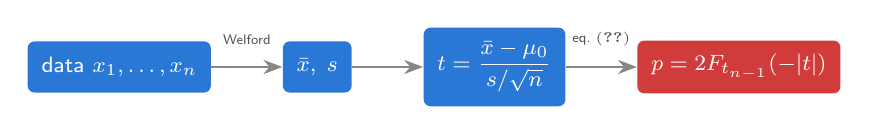
\begin{tikzpicture}[node distance=8mm and 9mm]
  \node[dist, fill=sBlue] (data) {data $x_1,\dots,x_n$};
  \node[dist, fill=sBlue, right=of data] (summ) {$\bar x,\; s$};
  \node[dist, fill=sBlue, right=of summ] (tstat)
    {$t=\dfrac{\bar x-\mu_0}{s/\sqrt n}$};
  \node[dist, fill=cRed, right=of tstat] (pval)
    {$p = 2F_{t_{n-1}}(-|t|)$};
  \draw[flow] (data) -- (summ)
    node[flowlab, pos=0.5, yshift=3.5mm] {Welford};
  \draw[flow] (summ) -- (tstat);
  \draw[flow] (tstat) -- (pval)
    node[flowlab, pos=0.5, yshift=3.5mm] {eq.~\eqref{eq:tcdf}};
\end{tikzpicture}
\end{center}

Figure~\ref{fig:rejection} shows the geometry on the library's own test
fixture (\S\ref{sec:tests}): ten measurements with mean $5.47$, tested
against $\mu_0=5$, give $t_{\text{obs}}=3.12$ on $9$ degrees of freedom
and $p=0.012$ --- the observed statistic sits well beyond the $5\%$
critical value, so either $H_0$ is false or a 1-in-80 coincidence
occurred.  The summaries themselves are computed by Welford's one-pass
recurrence \citep{welford1962}, which avoids the catastrophic cancellation
of the naive sum-of-squares formula.

\begin{figure}[htbp]
\centering
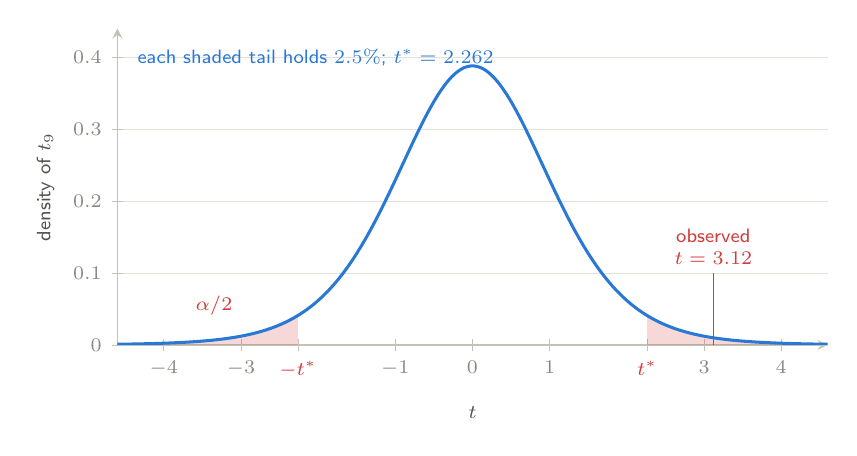
\begin{tikzpicture}
\begin{axis}[psaxis, xmin=-4.6, xmax=4.6, ymin=0, ymax=0.44,
    xlabel={$t$}, ylabel={density of $t_9$},
    domain=-4.6:4.6, samples=220,
    xtick={-4,-3,-1,0,1,3,4},
    extra x ticks={-2.262, 2.262},
    extra x tick labels={$-t^{*}$, $t^{*}$},
    extra x tick style={ticklabel style={color=cRed, font=\scriptsize}}]
  \addplot[draw=none, fill=cRed, fill opacity=0.20,
           domain=2.262157:4.6] {0.3880349*(1+x^2/9)^(-5)} \closedcycle;
  \addplot[draw=none, fill=cRed, fill opacity=0.20,
           domain=-4.6:-2.262157] {0.3880349*(1+x^2/9)^(-5)} \closedcycle;
  \addplot[sBlue] {0.3880349*(1+x^2/9)^(-5)};
  \draw[cRed, semithick] (axis cs:3.121,0) -- (axis cs:3.121,0.10);
  \node[pslabel, color=cRed, anchor=south, align=center]
    at (axis cs:3.121,0.105) {observed\\$t=3.12$};
  \node[pslabel, color=cRed, anchor=south] at (axis cs:-3.35,0.035)
    {$\alpha/2$};
  \node[pslabel, color=cRed, anchor=south] at (axis cs:3.35,0.035)
    {\phantom{$\alpha/2$}};
  \node[pslabel, color=sBlue, anchor=west] at (axis cs:-4.4,0.40)
    {each shaded tail holds $2.5\%$; $t^{*}=2.262$};
\end{axis}
\end{tikzpicture}
\caption{The one-sample $t$-test on the repository's own test fixture
($n=10$, $\mathrm{df}=9$).  Under $H_0$ the statistic follows the blue
$t_9$ density; the shaded tails beyond $\pm t^{*}$ are the $5\%$ rejection
region, and the observed $t=3.12$ lands past them, giving the two-sided
$p$-value $0.012$ --- the total tail area beyond $\pm 3.12$.\
\webfig{ttest}}
\label{fig:rejection}
\end{figure}

\srcref{src/stats.c: ps\_summarize(), ps\_t\_test\_one\_sample()}

\subsection{Welch's two-sample t-test}\label{sec:welch}

The commonest real question is comparative: do two groups --- treatment
and control, variant A and variant B --- share a mean?  With samples
$x_1,\dots,x_{n_x}$ and $y_1,\dots,y_{n_y}$, \citet{welch1947} tests
$H_0\colon \mu_X=\mu_Y$ with
\begin{equation}\label{eq:welch}
t=\frac{\bar x-\bar y}
       {\sqrt{s_x^2/n_x+s_y^2/n_y}},
\qquad
\nu \approx \frac{\bigl(s_x^2/n_x+s_y^2/n_y\bigr)^2}
       {\dfrac{(s_x^2/n_x)^2}{n_x-1}+\dfrac{(s_y^2/n_y)^2}{n_y-1}},
\end{equation}
the degrees of freedom being the Welch--Satterthwaite approximation
\citep{satterthwaite1946} --- generally fractional, which is why
\texttt{ps\_t\_test} carries \texttt{df} as a double.  Unlike the older
pooled test, Welch's does not assume the two variances are equal, and it
loses almost nothing when they happen to be; that robustness has made it
the default two-sample test in modern practice (and in R's
\texttt{t.test}).  It is the standard analysis for randomized experiments
and A/B tests; the same statistic inverted gives the confidence interval
for the difference in means that any experiment report should carry.

\srcref{src/stats.c: ps\_t\_test\_welch()}

\section{The driver and the tests}\label{sec:driver}

The repository ships two executables that turn the theory above into
running evidence: a driver that \emph{shows} the library working, and a
test suite that \emph{proves} it.

\subsection{Simulation meets theory}\label{sec:moments}

The driver (\texttt{make run}) simulates $200{,}000$ draws from each
distribution at the worked parameters of \S\ref{sec:discrete}--%
\S\ref{sec:continuous} and prints sample mean and variance beside the
theoretical $\E X$ and $\Var X$ --- the law of large numbers as a table
(excerpt from seed $20260718$):

\begin{center}\small
\begin{tabular}{lrrrr}
\toprule
distribution & mean & $\E X$ & variance & $\Var X$ \\
\midrule
Binomial$(20,0.25)$ & $5.008$  & $5$    & $3.733$  & $3.75$ \\
Poisson$(4)$        & $3.990$  & $4$    & $3.990$  & $4$ \\
Exponential$(0.5)$  & $1.995$  & $2$    & $3.985$  & $4$ \\
Normal$(10,2)$      & $10.001$ & $10$   & $3.985$  & $4$ \\
Gamma$(3,2)$        & $6.009$  & $6$    & $12.002$ & $12$ \\
Beta$(2,5)$         & $0.285$  & $0.286$& $0.0254$ & $0.0255$ \\
Student's $t_8$     & $-0.002$ & $0$    & $1.332$  & $4/3$ \\
$F_{5,12}$          & $1.201$  & $1.2$  & $1.077$  & $1.08$ \\
\bottomrule
\end{tabular}
\end{center}

\subsection{The t-tests, live}\label{sec:demos}

The driver then runs both tests of \S\ref{sec:inference} on data it has
just simulated --- a situation where, uniquely, we \emph{know} the truth.
A one-sample test of $N(10,2)$ data against its true mean ($H_0$ true)
yielded $p=0.44$: no false alarm.  A Welch test of $N(10,2)$ against
$N(11.5,3)$ ($H_0$ false) yielded $p=0.014$: difference detected.
Re-running with other seeds shows the expected behaviour: under a true
null the $p$-values scatter uniformly (occasionally below $0.05$ --- type
I error is a feature, not a bug), while under the false null they
concentrate near zero at this effect size and $n$.

\subsection{The test suite}\label{sec:tests}

\texttt{make test} runs about a hundred thousand checks in three layers,
in increasing order of subtlety.  \emph{Fixtures}: CDF, pmf and $t$-test
results are compared to reference values computed independently with
SciPy (each fixture's provenance is recorded beside it in the source).
\emph{Identities}: mathematical facts that must hold exactly, such as the
symmetry $I_x(a,b)+I_{1-x}(b,a)=1$ of equation~\eqref{eq:incbeta}, or
$P(\tfrac12,x)=\operatorname{erf}\sqrt{x}$ linking our incomplete gamma
to the C library's \texttt{erf}.  \emph{Statistical}: with a fixed seed,
every sampler's $200{,}000$-draw mean must land within five standard
errors of theory; and $2{,}000$ simulated one-sample $t$-tests under a
true null must reject at close to the nominal $5\%$ rate --- an
end-to-end check that samplers, special functions and test logic agree,
and an empirical verification of the uniform-$p$-value fact of
\S\ref{sec:uniform}.

\srcref{app/simulate.c \ and \ tests/test\_probsim.c}

\section{A modeler's cheat sheet}\label{sec:cheatsheet}

The table below compresses the tour into one glance: what each
distribution models, and the inference task where it most often appears.

\begin{center}\small
\begin{tabular}{lll}
\toprule
distribution & models & flagship inference role \\
\midrule
Bernoulli   & single yes/no event        & proportion estimation, A/B tests \\
Binomial    & successes in $n$ trials    & exact tests of proportions \\
Geometric   & failures until success     & retry/attrition modeling \\
Poisson     & rare-event counts          & count regression, goodness of fit \\
Uniform     & total ignorance on a range & $p$-values under $H_0$; simulation \\
Exponential & memoryless waiting time    & survival \& reliability baselines \\
Normal      & sums of small effects      & CLT; regression noise \\
Gamma       & accumulated waits, scales  & conjugate prior for rates \\
Beta        & unknown proportions        & conjugate prior for $p$; bandits \\
$\chi^2$    & summed squared noise       & variance CIs, GoF, likelihood ratios \\
Student $t$ & normalized small samples   & $t$-tests, robust models \\
$F$         & variance ratios            & ANOVA, regression $F$-tests \\
\bottomrule
\end{tabular}
\end{center}

For going further, three references span the territory:
\citet{devroye1986} for everything about generating non-uniform random
variables, \citet{knuth1997} for the theory of the uniform generators
underneath, and \citet{press1992} for the numerical special-function
craft of \S\ref{sec:special}.

\bibliographystyle{plainnat}
\bibliography{references}

\end{document}
